\documentclass[a4paper,10pt]{article}

\usepackage[a4paper,left=2.25cm,right=2.25cm,top=2.5cm,bottom=2.5cm]{geometry}

\title{Glassware Diagrams}
\author{David Roberts}
\date{}

% (c) 2007-2008 David Roberts

\usepackage{ifthen}
\newcommand{\ifnonzero}[2]{
 \ifthenelse{\equal{#1}{0}}{}{#2}
}

\usepackage{tikz}

\tikzstyle{glassware} = [fill=white]

\newcommand{\tripodheight}{5.3}
\newcommand{\testtubeheight}{3}

\newcommand{\bunsen}[2][]{
 \begin{scope}[shift={(#2)},glassware,#1]
  \filldraw (-1.55,0) -- (-1.55,0.2)  -- (-0.45,0.7)  -- (-0.45,1.4)  -- (0.45,1.4)
                  -- (0.45,0.7) -- (1.55,0.2) -- (1.55,0) -- cycle; % base
  \filldraw (-0.4,1.4) rectangle (0.4,3.8); % neck
  \filldraw (-0.45,3.8) rectangle (0.45,4.8); % head
 \end{scope}
}

\newcommand{\tripod}[2][]{
 \begin{scope}[shift={(#2)},glassware,#1]
  \filldraw (-2,0) -- (-1.3,5.1) -- (-1.8,5.1) -- (-1.8,5.3) -- (1.8,5.3)
               -- (1.8,5.1)  -- (1.3,5.1) -- (2,0) -- (1.8,0)
               -- (1.1,5.1) -- (-1.1,5.1) -- (-1.8,0) -- cycle;
 \end{scope}
}

\newcommand{\crucible}[2][]{
 \begin{scope}[shift={(#2)},glassware,#1]
  \draw (-0.7,1.4) .. controls (-0.7,1) and (-0.8,0) .. (-0.4,0)
     -- (0.4,0)    .. controls (0.8,0) and (0.7,1)  ..  (0.7,1.4);
 \end{scope}
}

\newcommand{\cruciblelid}[2][]{
 \begin{scope}[shift={(#2)},glassware,#1]
  \draw[shift={(0,1.4)}] (-0.8,-0.15) .. controls (-0.8,0.15) .. (-0.65,0.15)
     -- (0.65,0.15)   .. controls (0.8,0.15)  .. (0.8,-0.15);
 \end{scope}
}

\newcommand{\metalcoil}[2][]{
 \begin{scope}[shift={(#2)},glassware,#1]
  \filldraw (-0.3,0.1) rectangle (0.3,0.3);
  \filldraw (-0.3,0.1) -- (-0.3,0.3) arc (-90:-60:0.9) -- ++(-60:0.2) arc (-60:-90:1.1) -- cycle;
 \end{scope}
}

\newcommand{\dropper}[2][]{
 \begin{scope}[shift={(#2)},glassware,#1]
  \filldraw[rounded corners]
            (-0.1,0)  -- (-0.2,2.4)  -- (-0.3,2.7) -- (-0.35,4.5)
         -- (0.35,4.5)  -- (0.3,2.7)  -- (0.2,2.4)   -- (0.1,0) -- cycle;
 \end{scope}
}

\newcommand{\beaker}[3][]{
 \begin{scope}[shift={(#2)},glassware,#1]
  \draw[rounded corners]
        (-1.5,3) -- (-1.3,3) -- (-1.3,0) -- (1.3,0) -- (1.3,3) -- (1.5,3);
  \ifnonzero{#3}{
   \filldraw
        [yscale=2.8] (-1.3,#3)
        [rounded corners] -- (-1.3,0) -- (1.3,0)
        [sharp corners] -- (1.3,#3) -- cycle;
  }
 \end{scope}
}

\newcommand{\flask}[3][]{
 \begin{scope}[shift={(#2)},glassware,#1]
  \ifnonzero{#3}{
   \begin{scope}
    \clip[rounded corners]
         (-0.45,3) -- (-0.25,3) -- (-0.25,2) -- (-1.0,0) -- (1.0,0) -- (0.25,2) -- (0.25,3) -- (0.45,3);
    \filldraw
         [yscale=2.8] (-1.0,#3)
         [rounded corners] -- (-1.0,0) -- (1.0,0)
         [sharp corners] -- (1.0,#3) -- cycle;
   \end{scope}
  }
  \draw[rounded corners]
        (-0.45,3) -- (-0.25,3) -- (-0.25,2) -- (-1.0,0) -- (1.0,0) -- (0.25,2) -- (0.25,3) -- (0.45,3);
 \end{scope}
}

\newcommand{\testtube}[3][]{
 \begin{scope}[shift={(#2)},glassware,#1]
  \ifnonzero{#3}{
   \fill[yscale=2.8] (-0.3,#3) -- (-0.3,0.1071428571) -- (0.3,0.1071428571) -- (0.3,#3) -- cycle; % 0.1071428571 = 0.3/2.8
   \fill (-0.3,0.3) [rounded corners] -- (-0.3,0.3) arc (-180:0:0.3) -- (0.3,0.3) [sharp corners] -- (0.3,0.3) -- cycle;
   \draw[yscale=2.8] (-0.3,#3) -- (0.3,#3);
  }
  \draw[rounded corners]
        (-0.5,3) -- (-0.3,3) -- (-0.3,0.3) arc (-180:0:0.3) -- (0.3,3) -- (0.5,3);
 \end{scope}
}

\newcommand{\stopper}[2][]{
 \begin{scope}[shift={(#2)},glassware,#1]
  \filldraw (-0.35,0.3) -- (-0.25,-0.5) -- (0.25,-0.5) -- (0.35,0.3) -- cycle;
 \end{scope}
}

\newcommand{\pile}[2][]{
 \begin{scope}[shift={(#2)},glassware,#1]
  \filldraw (-0.3,0.1) -- (0.3,0.1) -- (0.1, 0.3) arc (45:135:0.141421) -- cycle; % 0.141421 = 0.2/sqrt(2)
 \end{scope}
}

\newcommand{\burette}[3][]{
 \begin{scope}[shift={(#2)},glassware,#1]
  \ifnonzero{#3}{
   \begin{scope}
    \clip[rounded corners]
         (-0.5,9) -- (-0.3,9) -- (-0.3,3) -- (-0.15,2.8) -- (-0.15,1) -- (0,0) -- (0.15,1) -- (0.15,2.8) -- (0.3,3) -- (0.3,9) -- (0.5,9);
    \filldraw[shift={(0,2.7)},yscale=6.1] (-0.5,#3) rectangle (0.5,0);
    \fill (-0.5,0) rectangle (0.5,2.7);
   \end{scope}
  }
  \draw[rounded corners]
        (-0.5,9) -- (-0.3,9) -- (-0.3,3) -- (-0.15,2.8) -- (-0.15,1) -- (0,0) -- (0.15,1) -- (0.15,2.8) -- (0.3,3) -- (0.3,9) -- (0.5,9);
  \filldraw[fill=white,rounded corners] (-0.3,2.7) rectangle (0.6,2.4);
  \filldraw[fill=white,rounded corners] (0.4,3.0) rectangle (0.6,2.1);
 \end{scope}
}


\begin{document}
 \maketitle
 
 \begin{figure}[h!]
  \begin{center}
   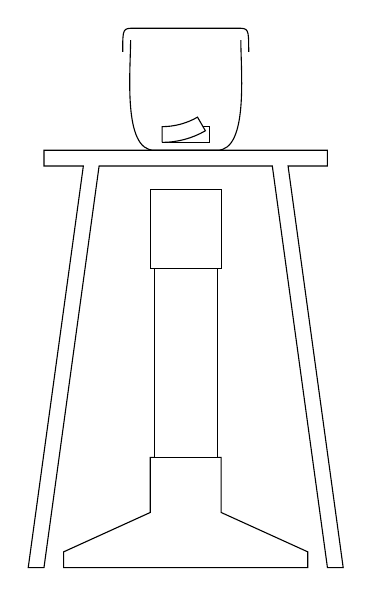
\begin{tikzpicture}
    \bunsen{0,0}
    \tripod{0,0}
    \crucible{0,\tripodheight}
    \cruciblelid{0,\tripodheight}
    \metalcoil{0,\tripodheight}
   \end{tikzpicture}
   \caption{Bunsen burner, tripod, crucible with lid, metal coil}
  \end{center}
 \end{figure}
 
 \begin{figure}[h!]
  \begin{center}
   \begin{tikzpicture}
    \dropper[rotate={-45}]{0,0}
   \end{tikzpicture}
   \caption{Dropper}
  \end{center}
 \end{figure}
 
 \begin{figure}[h!]
  \begin{center}
   \begin{tikzpicture}
    \beaker{0,0}{0}
   \end{tikzpicture}
   \caption{Empty beaker}
  \end{center}
 \end{figure}
 
 \begin{figure}[h!]
  \begin{center}
   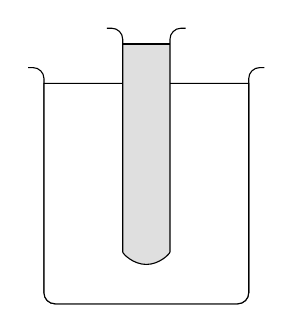
\begin{tikzpicture}
    \beaker{0,0}{1.00}
    \testtube[fill=gray!25]{0,0.5}{1.00}
   \end{tikzpicture}
   \caption{Test-tube in filled beaker}
  \end{center}
 \end{figure}
 
 \begin{figure}[h!]
  \begin{center}
   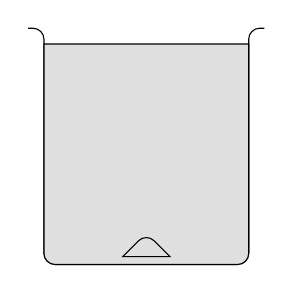
\begin{tikzpicture}
    \begin{scope}[shift={(0,0)}]
     \beaker[fill=gray!25]{0,0}{1.00}
     \pile[fill=gray!25]{0,0}
    \end{scope}
   \end{tikzpicture}
   \caption{Powder pile in filled beaker}
  \end{center}
 \end{figure}
 
 \begin{figure}[h!]
  \begin{center}
   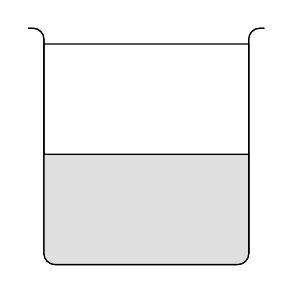
\begin{tikzpicture}
    \begin{scope}[shift={(0,0)}]
     \beaker{0,0}{1.00}
     \beaker[fill=gray!25]{0,0}{0.50}
    \end{scope}
   \end{tikzpicture}
   \caption{Beaker filled with mixture}
  \end{center}
 \end{figure}
 
 \begin{figure}[h!]
  \begin{center}
   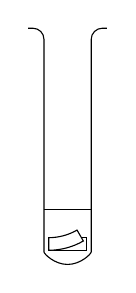
\begin{tikzpicture}
    \testtube{0,0}{0.25}
    \metalcoil[scale=0.8]{0,0.1}
   \end{tikzpicture}
   \caption{25\% filled test-tube with metal coil}
  \end{center}
 \end{figure}
 
 \begin{figure}[h!]
  \begin{center}
   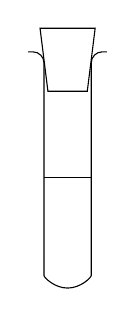
\begin{tikzpicture}
    \testtube{0,0}{0.50}
    \stopper{0,\testtubeheight}
   \end{tikzpicture}
   \caption{50\% filled test-tube with stopper}
  \end{center}
 \end{figure}
 
 \begin{figure}[h!]
  \begin{center}
   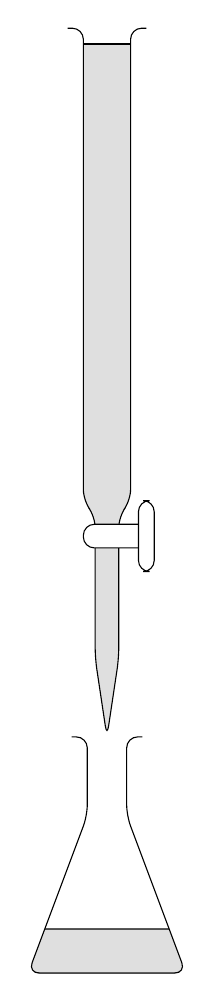
\begin{tikzpicture}
    \tikzstyle{glassware} = [fill=gray!25]
    \flask{0,0}{0.2}
    \burette{0,3}{1.0}
   \end{tikzpicture}
   \caption{Flask with burette}
   \label{d1}
  \end{center}
 \end{figure}
\end{document}
